\documentclass[12pt, a4paper, twoside]{article}
\usepackage[utf8]{inputenc}
\usepackage[T1]{fontenc}
\usepackage[dutch,english]{babel}
\usepackage[official]{eurosym}
\usepackage{graphicx}
\graphicspath{ {./images/} }
\usepackage{float}
\usepackage{xurl}
\usepackage{hyperref}
\hypersetup{colorlinks=true, linkcolor=blue, citecolor=blue, filecolor=blue, urlcolor=blue, pdftitle=, pdfauthor=, pdfsubject=, pdfkeywords=}
\usepackage{tabularx}
\usepackage{listings}
\usepackage{adjustbox}
\usepackage{color}

\title{Linux GUI Opdrachten}
\author{Dennis Leeuw}
\date{\today}

\begin{document}

\begin{titlepage}
\maketitle
\end{titlepage}

\begin{abstract}
Dit document bevat de opdrachten die behoren bij het Linux GUI document
\end{abstract}

\section{VirtualBox Installatie}
Download VirtualBox voor jouw besturingssysteem van \url{https://www.virtualbox.org/} en installeer het op je machine.


\section{Bestanden en programma's}
Start de LibreOffice Writer applicatie op.

Neem de tekst over uit de plaat in figuur \ref{fig:LOWriter_tekst} en zorg dat deze tekst een hoofdstuk titel wordt door de stijl te
veranderen. We gaan het document later vullen. Selecteer File en Save as{\dots} om het bestand op te slaan met als naam:
Document1. Sluit daarna LibreOffice Writer weer af.

\begin{figure}[H]
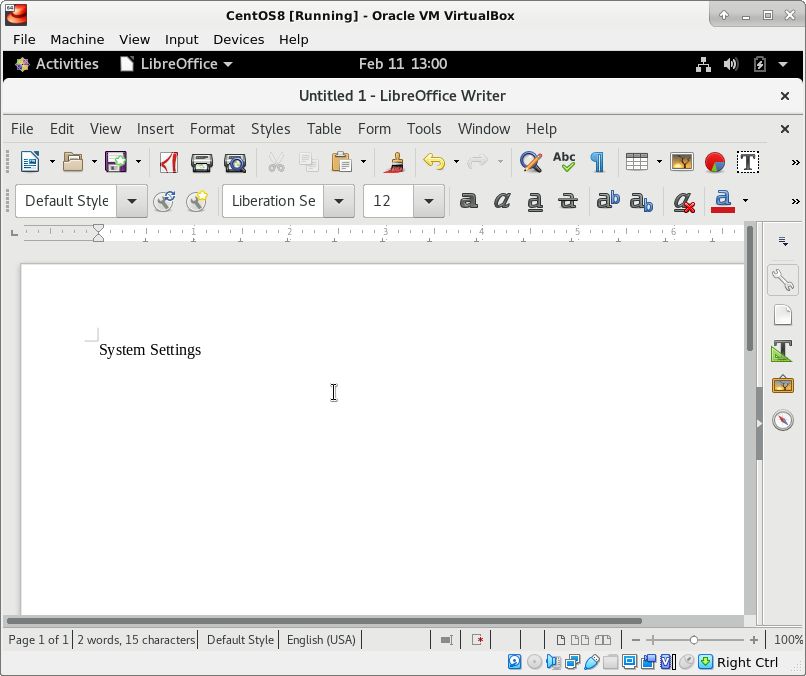
\includegraphics[width=0.9\textwidth]{linuxreader-img015.png}
	\caption{LibreOffice Writer met een eerste tekts}
	\label{fig:LOWriter_tekst}
\end{figure}


\section{Software}
Installeer GIMP op je systeem


\section{E-mail Clients}
Start Evolution op, koppel een GMail account aan evolution door gebruik te maken van het IMAP protocol en stuur een e-mail aan een medestudent.


\end{document}

